\chapter{Position Feedback}
\section{Overview}
This section discusses the position feedback sub-system of the autonomous `mouse'. The position feedback within the `mouse' control loop is responsible for detecting the mouse's approximate location in relation to the track wire and providing a position feedback signal for steering correction. The current circuit design utilises inductive pick-up coils to sense the AC magnetic flux generated by a trackwire conducting at \(20\) kHz \(\simeq1\) A. The induced voltage signal is subsequently processed by filtering, amplification and peak detector stages to produce a DC feedback signal \cite{Robinson2025}.

A key focus of this section is to address one of the limitations identified in the original sensing sub-system design: the requirement for a dual power supply to bias the operational amplifier appropriately to process a \(100\) mVpp AC signal. This dependency increases the number of batteries required, increasing the `mouse' weight and the project's environmental impact by increasing e-waste. This section aims to explore and implement alternative circuit configurations capable of operating from a single supply of \(9\) V DC. The proposed solutions must maintain signal integrity and compatibility with downstream control systems. The designs must be evaluated on performance, simplicity, and cost of implementation.

\section{Design Concepts and Methods}

\subsection{Design A: Voltage Divider}
Design A (Fig.\ref{fig:vol_div_theory}) employs a voltage divider to proportionally split the \(9\) V input supply voltage to create a new virtual GND. The division is done across two or more resistive sources (see Fig.\ref{fig:vol_div_theory}) with the output voltage dependent on the ratio between the component's impedances. The resulting output voltage equation (Eq.\ref{equ:vol_div}) is derived using Kirchhoff's Voltage Law and Ohm's Law, where \(Z_1\) and \(Z_2\) are impedances of the two components shown in Fig.\ref{fig:vol_div_theory}. The impedance ratio in Design A is set at \(1:1\) resulting in a \(4.5\) V virtual GND

\begin{equation}
    V_{Out}=\frac{Z_2}{Z_1+Z_2}*V_s
    \label{equ:vol_div}
\end{equation}

\begin{figure}[H]
    \centering
    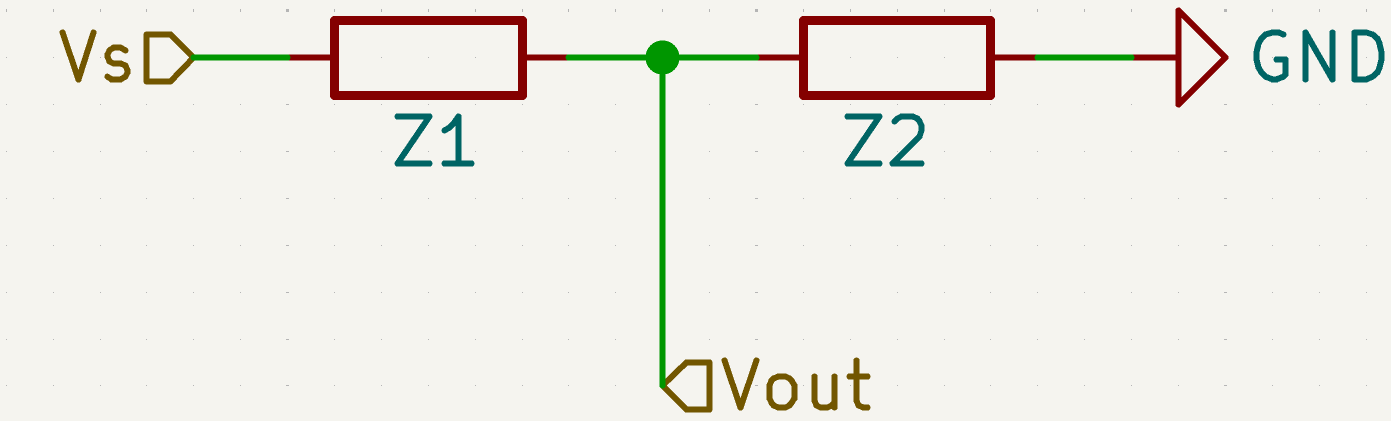
\includegraphics[width=0.7\textwidth]{circuits/volt_div.png}
    \caption[Simple Voltage Divider]{Voltage divider circuit with two resistive components, \(V_s\) is the supply voltage and \(V_{out}\) is the reduced voltage reference.}
    \label{fig:vol_div_theory}
\end{figure}

The new \(4.5\) V virtual GND becomes the new reference point for the operational amplifier and input signal. The operational amplifier and input signal will treat the \(4.5\) V reference as its GND. Biasing the operational amplifier and input signal this way allows the supply rails to be at \(9\) V (\(+ve\) supply) and \(0\) V (\(-ve\) supply), and allows for the use of a single power supply, however the operational amplifier is now operated with a \(\pm4.5\) V supply halving amplification potential. Therefore, an AC-coupled input signal will not reduce the inputs below the \(-ve \) supply rail and cause the operational amplifier to malfunction.

\subsection{Design B: 555 Timer with Negative Charge Pump}
Design B (Fig.\ref{fig:555_ti}) utilises a 555 timer circuit in an astable configuration to generate a rectangular wave output, which drives a negative charge pump circuit. This arrangement allows the generation of a negative voltage supply from a single positive \(9\) V voltage source.

\subsubsection{Astable 555 Timer Operation}

The 555 timer's oscillation frequency is determined by the values of two resistors (\(R_a\) and \(R_b\)) and one capacitor (\(C\)) as shown in Fig.\ref{fig:555_ti}. The resulting output is a square wave with frequency calculated using Eq.\ref{equ:555_frq} as defined by Texas Instruments \cite[p.12]{TI_NE555}.
\begin{equation}
    \label{equ:555_frq}
    f =\frac{1.44}{(R_a+2R_{b})*C}
\end{equation}

The duty cycle of the astable output can be calculated using Eq.\ref{equ:555_duty} as defined by Texas Instruments \cite[p.12]{TI_NE555}.

\begin{equation}
    \label{equ:555_duty}
    Duty =\frac{R_a+R_{b}}{R_a+2R_{b}}*100\%
\end{equation}

\begin{figure}[H]
    \centering
    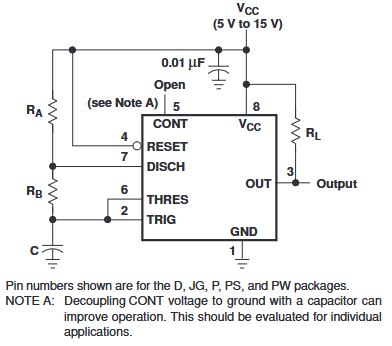
\includegraphics[width=0.7\textwidth]{circuits/555_TI.png}
    \caption[Astable 555 Timer Circuit]{Astable 555 timer circuit configuration showing component connections and pin assignments \cite[p.12]{TI_NE555}. The circuit illustrates the standard configuration for generating rectangular wave outputs with frequency determined by \(R_A\), \(R_B\), and \(C\) values.}
    \label{fig:555_ti}
\end{figure}

\subsubsection{Negative Charge Pump Circuit}
The negative charge pump takes the oscillating output from the 555 timer and converts it to a negative DC voltage through a network of capacitors and diodes (Fig.\ref{fig:negcharge_theo}) as described by Horowitz and Hill \cite[pp.638-639]{Horowitz_Hill_AoE}.

The circuit operates by alternately charging and discharging capacitors through the diodes following the input waveform transitions. When the input signal (\(V_s\)) transitions to a high state, capacitor C1 charges through diode D2 towards GND. Diode D1 remains reverse-biased in this state, preventing current flow towards the output stage. As \(V_s\) switches to a low state, the voltage at the left side of C1 falls below GND potential. This voltage shift forward-biases diode D1, allowing charge to transfer to capacitor C2, which stores the accumulated negative voltage.

During each subsequent cycle of \(V_s\), the additional charge is transferred to C2, gradually increasing the magnitude of the negative output voltage at \(V_{neg}\). Diode D2 prevents the backflow of current during the low phase of \(V_s\), ensuring efficient charge transfer in one direction. The steady-state negative voltage developed across C2 depends on the amplitude of \(V_s\), the capacitance values of C1 and C2, the forward voltage drops of D1 and D2, and the switching frequency of the input signal.

\begin{figure}[H]
    \centering
    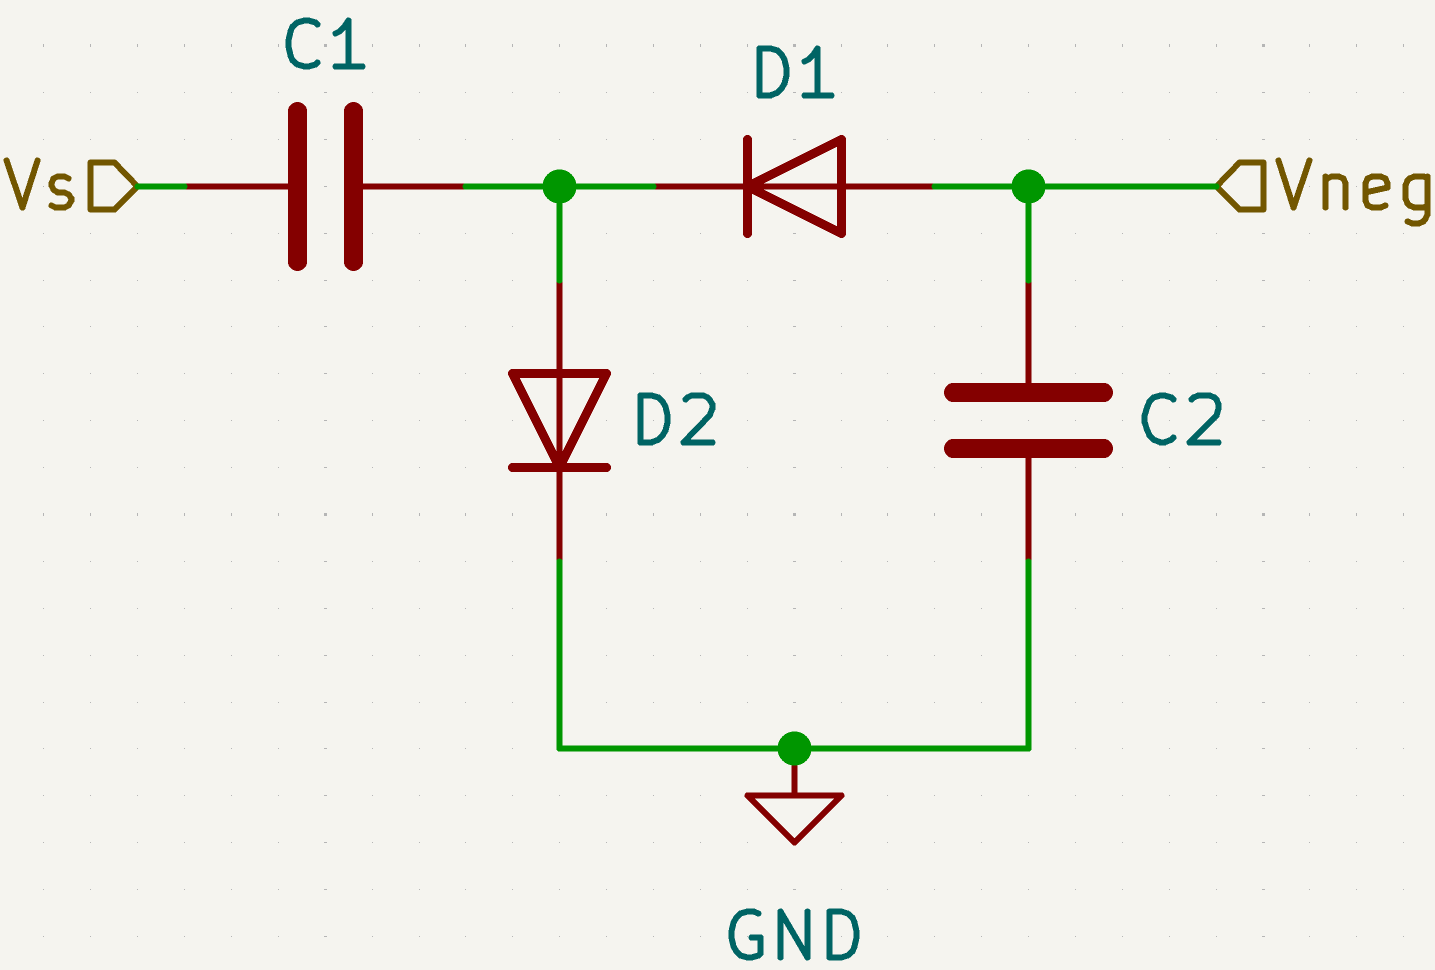
\includegraphics[width=0.6\textwidth]{circuits/neg_charge.png}
    \caption[Negative Charge Pump Circuit]{Schematic of a negative charge pump circuit using a pair of diodes and two capacitors. The circuit generates a negative output voltage (\(V_{neg}\)) from a positive square wave input (\(V_s\)) by transferring charge through C1 and rectifying the output via D1 and D2. Capacitor C2 acts as an output reservoir, smoothing the generated negative voltage.}
    \label{fig:negcharge_theo}
\end{figure}

The voltage efficiency of the charge pump under load can be defined as shown in Eq.\ref{eq:efficincee} where \(V_{neg}\) is the output voltage and \(Vs\) is the supply voltage.

\begin{equation}
\label{eq:efficincee}
    \eta=\frac{-(V_{neg})}{V_s}
\end{equation}

The negative charge pump creates a virtual negative voltage rail relative to the system GND. This new virtual negative rail and the \(9\) V power supply are used as the power rails for an operational amplifier. This setup allows the operational amplifier to have a dual supply from a single positive power supply, enabling regular signal processing operation.

\subsection{Design C: Precision Diode Clamping}
\begin{figure}[H]
    \centering
    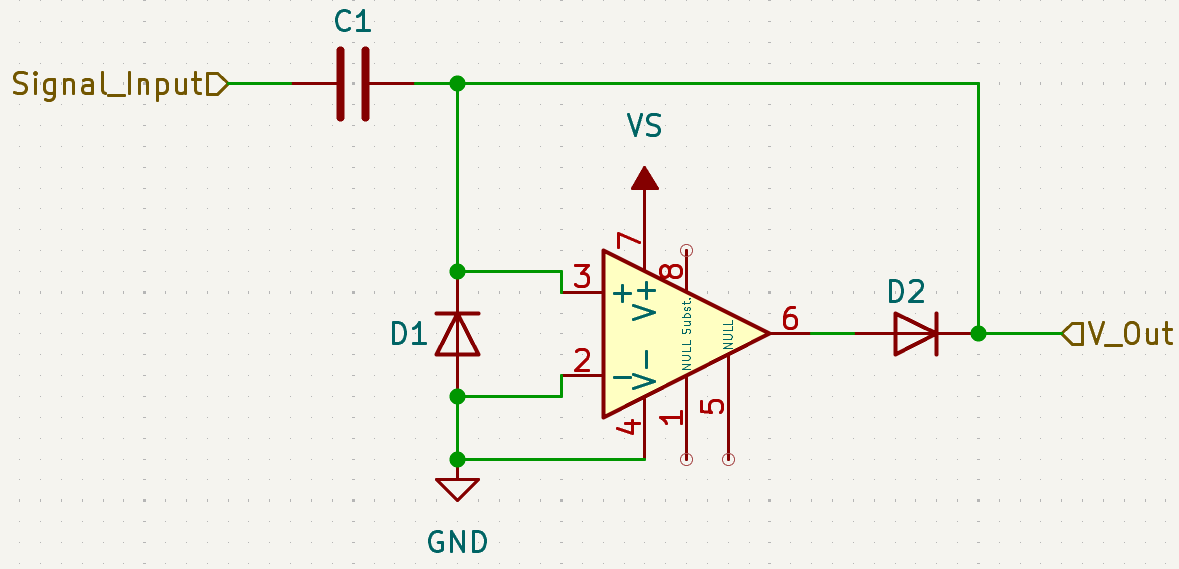
\includegraphics[width=0.8\textwidth]{circuits/prec_diode_clamp.png}
    \caption[Precision Diode Clamper Circuit]{Schematic of a precision diode clamper.}
    \label{fig:precidiode_clamp}
\end{figure}

Design C utilised a precision diode clamping circuit (Fig.\ref{fig:precidiode_clamp}) to clamp the voltage level of the input signal above \(0\) V and hence above GND. When the `Signal\_Input' drops below zero, the diode becomes forward-bias and allows current to pass, causing the capacitor to charge to the voltage level of the negative peak. The diode switches off once the input voltage rises back into the positive range, preventing further current flow. The charged capacitor then effectively adds its stored voltage to the input signal, shifting the entire waveform upward. As a result, the negative portions of the signal are raised closer to zero volts or higher. By pulling the signal above \(0\) V the signal can be amplified by an operational amplifier with supply rails at \(9\) V (\(+ve\) supply) and \(0\) V (\(-ve\) supply) allowing for the use of a single power supply. The effectiveness of this method depends on the characteristics of the operational amplifier used.


\section{Procedures}
\subsection{Design A: Voltage Divider}
\label{sec:volt_div}
\subsubsection{Assembly}

\begin{figure}[H]
    \centering
    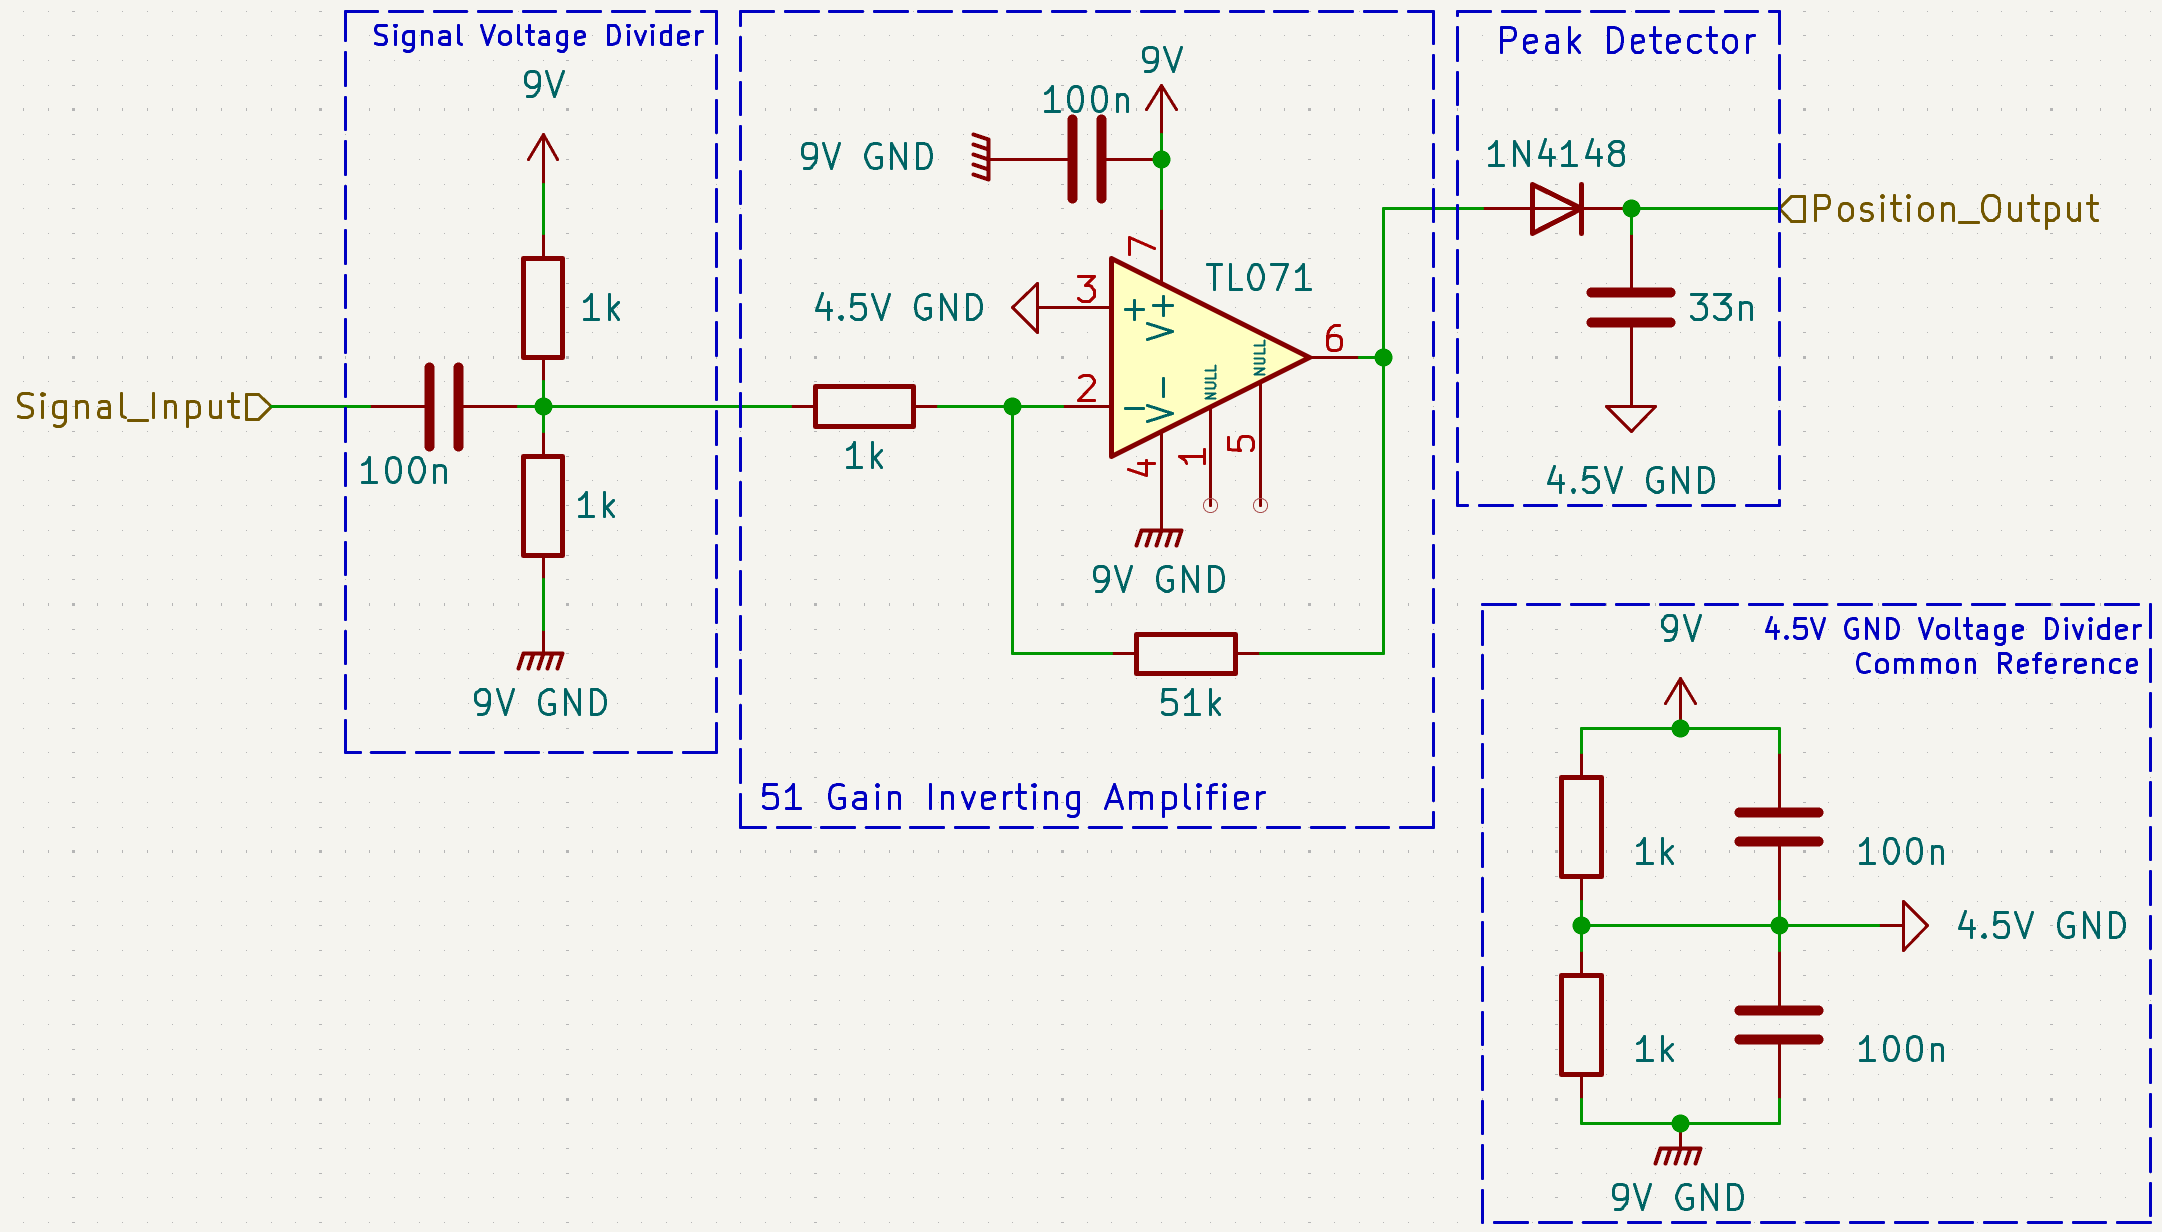
\includegraphics[width=1\linewidth]{circuits/volt_div_possub.png}
    \caption[Design A: Schematic]{Schematic of Design A. Including a voltage divider signal conditioning circuit with a 4.5 V virtual GND, ×51 inverting amplifier, and peak detector, powered from a single 9 V DC supply.}
    \label{fig:vol_div_circuit}
\end{figure}

Design A was built on a standard RH-32 breadboard following the design outline in Fig.\ref{fig:vol_div_circuit}. Firstly, the TL071 \cite{TI_TL071} operational amplifier was inserted into the breadboard and was configured in an inverting arrangement with a gain factor (\(A_v\)) of -51 (Eq.\ref{equ:inverting_amp}), the gain was set by the \break \(51\) k\(\Omega\) feedback resistor (\(R_f\)) and \(1\) k\(\Omega\) input resistor (\(R_{in}\)).

\begin{equation}
    \label{equ:inverting_amp}
    A_v = -\frac{R_f}{R_{in}}
\end{equation}

All connections made to the inverting input (pin 2) were as short as possible to reduce parasitic capacitance as suggested by Texas Instruments \cite[p.36]{TI_TL071}. The \(9\) V DC E3631A lab power supply was connected to pin 7 (\(+ve\) supply rail) with a \(100\) nF decoupling capacitor. The 9 V GND was then connected to pin 4 (\(-ve\) supply rail).

Secondly, a voltage divider circuit was constructed to create the \(4.5\) V GND (virtual GND). As shown in Fig.\ref{fig:vol_div_circuit} two \(1\) k\(\Omega\) resistors were connected in parallel with two \(100\) nF capacitors, the input of the voltage divider was connected to the  \(9\) V DC E3631A lab power supply and the \(9\) V GND was connected to the bottom. The output \(4.5\) V virtual GND was then taken from the central connection as seen in Fig.\ref{fig:vol_div_circuit}. The new \(4.5\) V virtual GND was then connected to the non-inverting input of the TL071.

Third, a voltage divider circuit was constructed to bias the input signal. As shown in Fig.\ref{fig:vol_div_circuit} two \(1\) k\(\Omega\) resistors were connected in series connecting the  \(9\) V DC E3631A lab power supply and the \(9\) V GND. The `Signal\_Input' was then coupled with a \(100\) nF capacitor at the centre point of the resistor and then further connected to the \(1\) k\(\Omega\) resistor (\(R_{in}\)).

Finally, a simple peak detector was assembled after the TL071 using a 1N4148 \cite{Vishay_1N4148} and \(33\) nF capacitor. The peak detector was constructed as shown in Fig.\ref{fig:vol_div_circuit} with the output of the TL071 connecting to the anode of the diode and the GND connection of the capacitor being connected to the \(4.5\) V virtual GND.

\subsubsection{Testing}
The steps for Testing Design A are as follows:

\begin{enumerate}
    \item \(9\) V, \(4.5\) V virtual GND and \(9\) V GND were verified using a KeySight 34450A multimeter.
    \item The Position\_Output DC voltage was measured three times using a KeySight 34450A multimeter when no input signal was applied to check for a potential failure mode, the values were then averaged. 
    \item The AFG2021 signal generator was turned on, set to high impedance and connected to `Signal\_Input' with GND connected the \(4.5\) V virtual GND. Additionally, a filtering capacitor of \(100\) nF was connected between the Signal\_Input and GND to reduce noise, which wouldn't be included in the final design as the signal normally comes from an LC filtered source. The output signal parameters were a Sine Wave set to \(20\) kHz frequency and \(100\) mVpp amplitude.
    \item{
    The KeySight DSO1014A oscilloscope was connected to Design A, making sure the oscilloscope probe ratio matched the input signal ratio and probe points were as close as possible to the measurement point:
    \begin{itemize}
        \item Channel 1: Output of AFG2021 Signal Generator
        \item Channel 2: TL071 pin 6 with probe reference connected to \(4.5\) V Common Reference
        \item Channel 3: `Position\_Output' with probe reference connected to \(4.5\) V Common Reference
    \end{itemize}
    }
    \item The steady-state \(100\) mV waveform was observed and stored on an external USB as a CSV for later analysis in Excel.

    \item The oscilloscope probes were then removed, and the KeySight 34450A multimeter was connected. The positive probe connected to `Position\_Output' and the reference probe to Design A's Common Reference.

    \item The steady-state DC voltage at \(100\) mVpp was recorded three times. The amplitude of the input signal was reduced by \(10\) mVpp and the new steady-state voltage was recorded in Microsoft Excel. This reduction of \(10\) mVpp was repeated till the amplitude reached \(20\) mVpp.
\end{enumerate}

All measurements were taken after a 5-second stabilisation period to minimise transient effects and were conducted at room temperature (approximately 22°C). The oscilloscope output was imported into Excel and used to generate graphs for analysis. The multimeter readings were tabulated and analysed; linear regression was performed to evaluate the system’s gain and linearity.

\subsection{Design B: 555 Timer and Negative Charge Pump}
\label{sec:2}
\subsubsection{Assembly}

\begin{figure}[H]
    \centering
    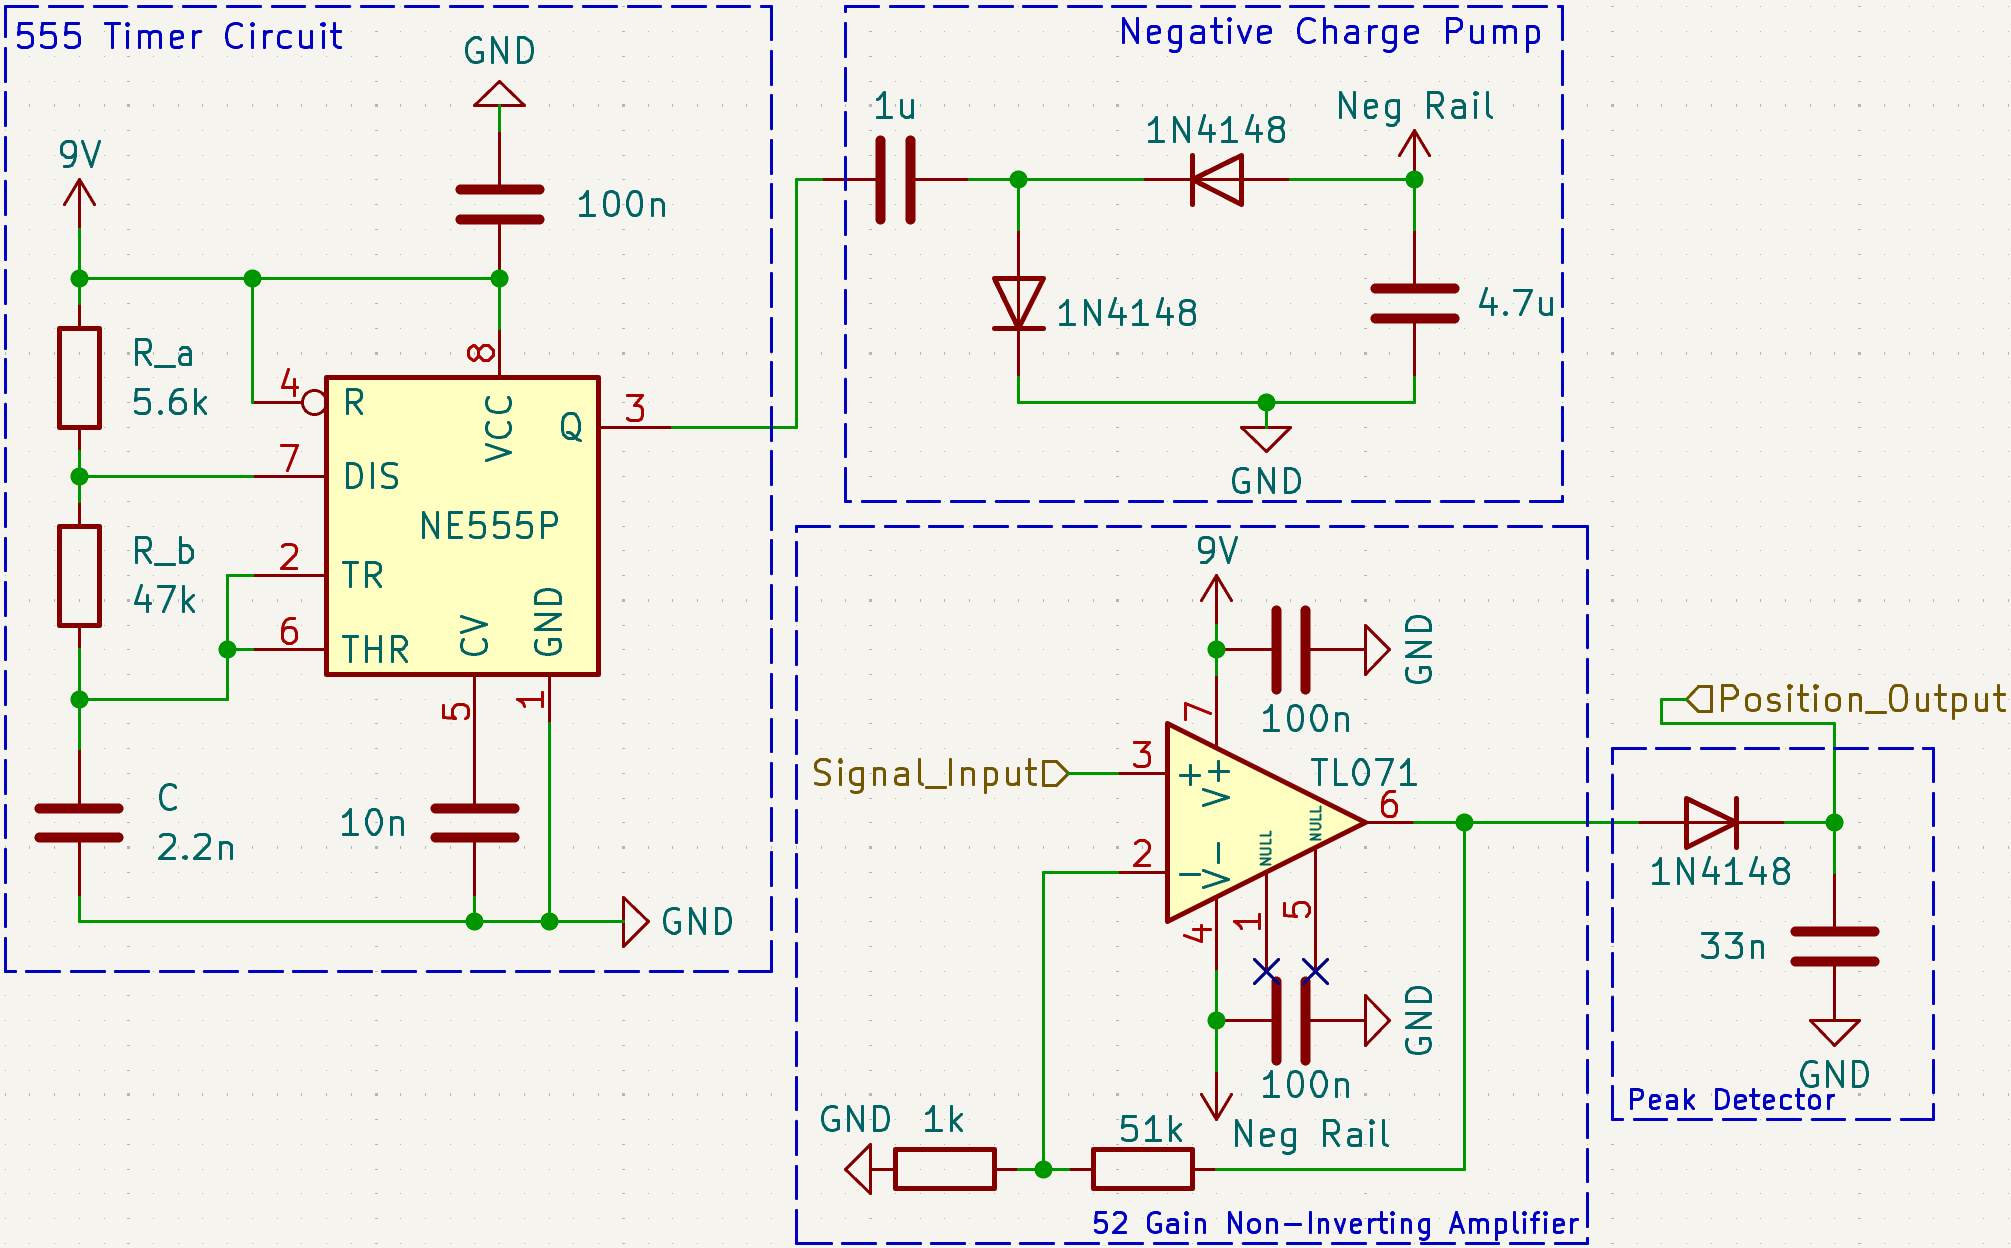
\includegraphics[width=1\linewidth]{circuits/555_possub.png}
    \caption[Design B: Schematic]{Schematic of Design B. Including a 555 astable timer with negative charge pump powered and x52 Non-inverting amplifier, powered from a single 9V DC supply.}
    \label{fig:555_circuit}
\end{figure}

Design B was built on a standard RH-32 breadboard following the design outline in Fig.\ref{fig:555_circuit}. Firstly, the astable mode 555 timer circuit was built using a NE555P \cite{TI_NE555}, the timing components being a \(5.6\) k\(\Omega\) (\(R_a\)), \(47\) k\(\Omega\) (\(R_b\)) and \(1\) nF (\(C\)) as shown in Fig.\ref{fig:555_circuit} following the naming convention used by Texas Instruments \cite[p.12]{TI_NE555}. The timing components selected create an oscillation frequency of \(14.46\) kHz. In addition, a \(10\) nF decoupling capacitor was placed between pin 5 (Control) and GND to improve stability as seen in Fig.\ref{fig:555_circuit} and suggested by Texas Instruments \cite[p.12]{TI_NE555}. Furthermore, during assembly, the timing capacitor and decoupling capacitors were placed as close as possible to the LM555 as advised to reduce possible parasitic capacitance. The \(9\) V DC E3631A lab power supply was connected to pins 4, 8 and the top of \(R_a\); the \(9\) V supply additionally had a \(100\) nF decoupling capacitor. After the 555 timer construction the accompanying negative charge pump circuit was built as seen in Fig.\ref{fig:555_circuit} using two 1N4148 diodes and two capacitors of values \(1\) \(\mu\)F and \(4.6\) \(\mu\)F.

Following on the TL071 operational amplifier \cite{TI_TL071} was inserted into the breadboard and was configured in a non-inverting arrangement with a gain factor (\(A_v\)) of gain factor of 52 (Eq.\ref{equ:noninverting_amp}) the gain was set by the \(51\) k\(\Omega\) feedback resistor(\(R_{f}\)) and \(1\) k\(\Omega\) GND resistor (\(R_{GND}\)). 

\begin{equation}
    \label{equ:noninverting_amp}
    A_v = 1+\frac{R_f}{R_{GND}}
\end{equation}


Again, all connections made to the inverting input (pin 2) were as short as possible, as mentioned in Section \ref{sec:volt_div}. The \(9\) V DC E3631A lab power supply was connected to pin 7 (\(+ve\) supply rail) and the negative charge pump output was connected to pin 4 (\(-ve\) supply rail); both supply rails had \(100\) nF decoupling capacitors.

\subsubsection{Testing}
Firstly, the DC \(9\) V, negative charge pump supply rail and \(9\) V GND were verified using a KeySight 34450A multimeter. The testing method for Design B followed the same procedure as outlined in Section \ref{sec:volt_div} steps \(2\rightarrow7\). All measurements were taken under the same conditions and analysed accordingly as defined in \ref{sec:volt_div}.

\subsection{Design C: Precision Diode Clamping}
\label{sec:3}
Design C was considered but ultimately not physically tested as the low input voltage range [0,100 mV] could not properly forward bias the input diode and risked pulling the inverting input of the operational amplifier below the available negative rail (\(0\) V). This would have resulted in the TL071 operational amplifier operating outside its recommended input range, potentially compromising circuit performance and reliability.

\section{Results}
\subsection{Design A: Voltage Divider}

\begin{table}[h]
    \centering
    \caption[Design A: Supply and Ground Measurements]{Measured DC \(9\) V supply rail and \(4.5\) V virtual GND relative to circuit GND. The potential difference between the circuit GND and the power supply GND was also recorded.}
    \begin{tabular}{|c|c|}
        \hline
        Measurment Point & Measured 3s.f.(V) \\ \hline\hline
        9 V Supply Rail & 8.99 \\ \hline
        4.5 V Virtual GND & 4.49 \\ \hline
        GND & \(6.68*10^{-4}\) \\ \hline
    \end{tabular}
    \label{tab:voltdiv_verification}
\end{table}

The voltage divider was verified at three key points: 9V Supply Rail, 4.5V Virtual GND and GND, as shown in Table \ref{tab:voltdiv_verification}:
\begin{itemize}
    \item \textbf{DC 9 V input}: The output voltage was measured at \(8.99\) V, showing a negligible deviation from the expected value.
    \item \textbf{4.5 V Virtual GND}: The measured voltage was \(4.49\) V, displaying a minimal difference from the theoretical result.
    \item \textbf{0 V (GND)}: The measured voltage was measured at \(6.68 * 10^{-4}\) V ,  approximating to zero confirming correct operation near GND.
\end{itemize}

As summarised in Table \ref{tab:voltdiv_verification}, these results indicate that the voltage divider functioned as expected. When Design A was tested at a 0Vpp input signal the `Position\_Output' remained stable at \(40\) mV.

\begin{figure}[H]
    \centering
    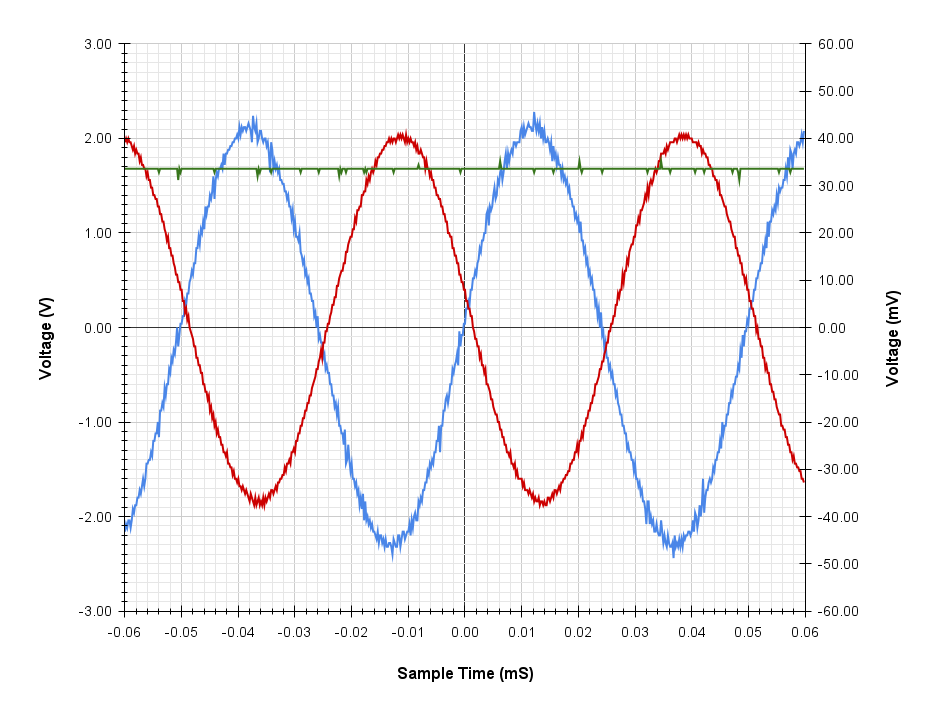
\includegraphics[width=1\linewidth]{graphs/voltagedivider_osciliscope.png}
    \caption[Design A: Oscilloscope Output with input signal of 100mVpp]{Graph showing Design A behaviour at \(100\) mVpp. The traces are the Signal Generator output (Channel 1: Blue), TL071 Operational Amplifier output (Channel 2: Red), and `Position\_Output' (Channel 3: Green) plotted against time (mS). The Signal Generator output is plotted on the right Y-axis in millivolts (mV), while the operational amplifier and Position Output are plotted on the left Y-axis in volts (V).}
    \label{fig:voltdiv_oscilloscope}
\end{figure}

The DSO1014A oscilloscope captured three signals: the `Signal\_Input' (Channel 1), the output of the TL071 operational amplifier (Channel 2), and the `Position\_Output' (Channel 3), as shown in Fig.\ref{fig:voltdiv_oscilloscope}.

\begin{itemize}
    \item \textbf{`Signal\_Input'}: The input sinusoidal waveform with a frequency of \(20\) kHz had peak values ranging from \(-48.8 \) mV to \(45\) mV hence a \(96\) mVpp signal. This indicates a discrepancy in the signal generator output signal and the observed peak-to-peak value.
    \item \textbf{TL071 Output}: The observed output signal inverts the input signal and exhibited peak values of approximately -1.8 V and 2 V, indicating a lower-than-expected gain of \(\approx-42\).
    \item \textbf{`Position\_Output'}: The output of the peak detector shows a steady DC value of approximately 1.7 V. This value is slightly lower than the peak value of the amplified signal (approximately 2 V), due to the voltage drop across the peak detector diode.
    
\end{itemize}

Overall, the oscilloscope graph in Fig.\ref{fig:voltdiv_oscilloscope} confirms that the operational amplifier is amplifying the input signal, though at a lower gain than intended. The peak detector captures a value slightly lower than the peak voltage but still approximately tracks the signal's maximum value.

\begin{figure}[H]
    \centering
    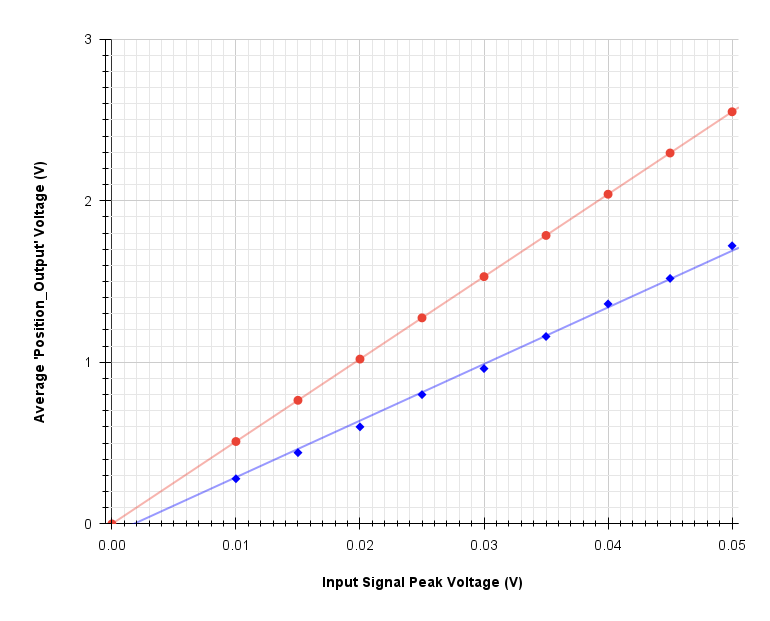
\includegraphics[width=1\linewidth]{graphs/voltagedivider_fullrange.png}
    \caption[Design A: Input Range Response]{Graph of Design A Input Signal Peak Voltage (V) against observed `Position\_Output' (V). Average observed output voltage is represented in Blue, and predicted output voltage is represented in Red.}
    \label{fig:voltdiv_fullrange}
\end{figure}

Fig.\ref{fig:voltdiv_fullrange} demonstrates the relationship between the input peak voltage and the observed output voltage within Design A. As shown in Fig.\ref{fig:voltdiv_fullrange}, the output voltage increases proportionally with the input peak voltage, following a near-linear trend as expected for a fixed-gain inverting amplifier circuit. However, the observed output values were consistently lower than the theoretical values predicted by the amplifier’s nominal gain setting of 51, indicating a reduction in observed gain within the circuit.

The maximum observed voltage was \(1.721\) V and a minimum observed voltage of \(0.280\) V. It should also be noted that the linear trend does not cross through the origin but crosses the x-axis at \(\approx0.002\) V.

These observations confirm the amplifier's overall linear behaviour and highlight the practical limitations demonstrated by the difference between the theoretical gain and the observed gain.

\subsubsection{Cost of Implementation}
\begin{table}[H]
    \centering
    \caption{Alphabetically Ordered Estimated Component Costs for Design A}
    \begin{tabular}{|l|c|c|c|}
    \hline
    \textbf{Component} & \textbf{Quantity} & \textbf{Unit Price (£)} & \textbf{Total Price (£)} \\ \hline\hline
    100nF Ceramic Disc Capacitor (50V) \cite{rs_100nfcap} & 4 & 0.17& 0.68\\ \hline
    1kΩ Resistor \cite{rs_1kresistor} & 5 & 0.162& 0.81\\ \hline
    1N4148 Signal Diode \cite{rs_1n4148} & 1 & 0.01& 0.01\\ \hline
    33nF Capacitor (Polyester, 100V) \cite{rs_33nfcap} & 1 & 0.122& 0.122\\ \hline
    51kΩ Resistor \cite{rs_51kresistor} & 1 & 0.054& 0.054\\ \hline
    9V Battery (RS PRO Alkaline) \cite{rs_9vbattery} & 1 & 2.08& 2.08\\ \hline
    TL071 Op-Amp (Single BiFET) \cite{rs_tl071} & 1 & 0.45& 0.45\\ \hline\hline
    \textbf{Total Estimated Cost} &&&\textbf{£4.21}\\ \hline
    \end{tabular}
    \label{tab:component_info_da}
\end{table}

Table \ref{tab:component_info_da} details the individual components required to implement Design A, alongside their quantities, specifications and unit costs based on UK-sourced pricing at the time of writing. The cost of implementation within the `mouse' would be £5.68, adding an additional inverting amplifier, peak detector and signal voltage divider. The cost difference between the original sub-system (Appendix \ref{app:mouseecost_og}) is -£1.70 a reduction of \(23\%\).

\subsection{Design B: 555 Timer and Negative Charge Pump}
\begin{table}[h]
    \centering
    \caption[Design B: Supply and Ground Measurements]{Measured \(9V\) supply rail and charge pump negative supply rail relative to the circuit GND. The potential difference between circuit GND and E3631A lab power supply GND was also recorded to verify correct internal biasing and GND reference stability within the single-supply configuration.}
    \begin{tabular}{|c|c|}
        \hline
        Measurement Point & Measured 3s.f.(V) \\ \hline\hline
        9 V Supply Rail & 8.99 \\ \hline
        Negative Rail & -5.50 \\ \hline
        GND & \(8.22*10^{-4}\) \\ \hline
    \end{tabular}
    \label{tab:555_verification}
\end{table}

The 555 timer design was verified at three key points: 9 V Supply Rail, Negative Supply Rail, and GND, as shown in Table \ref{tab:555_verification}:
\begin{itemize}
    \item \textbf{9 V input}: The output voltage was measured at \(8.99\) V, showing a negligible deviation from the expected value.
    \item \textbf{Negative Rail}: The measured voltage was \(-5.50\) V, displaying an efficiency of \break \(\frac{-5.50}{9}\approx 61.1\%\). Measured under circuit load.
    \item \textbf{0 V (GND)}: The measured voltage was measured at \(8.22*10^{-4}\) V, approximating to zero confirming correct operation near GND.
\end{itemize}

As summarised in Table \ref{tab:555_verification}, these results indicate that the 555 timer design functioned as expected. In addition, when Design B was tested at a 0Vpp input signal the `Position\_Output' remained stable at \(40\) mV.


\begin{figure}[H]
    \centering
    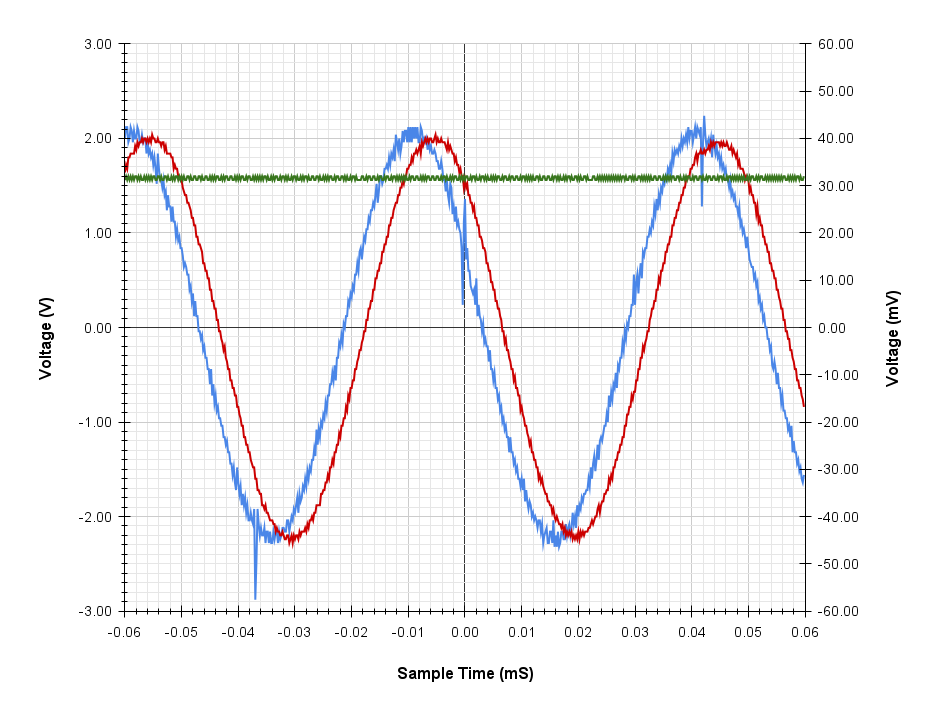
\includegraphics[width=1\linewidth]{graphs/555_osciliscope.png}
    \caption[Design B: Oscilloscope Output with input signal of 100mVpp]{Graph showing Design B behaviour at \(100\) mVpp. The traces are Signal Generator output (Channel 1: Blue), TL071 Operational Amplifier output (Channel 2: Red), and `Position\_Output' (Channel 3: Green) plotted against time (\(mS\)). The Signal Generator output is plotted on the right Y-axis in millivolts (mV), while the operational amplifier and Position Output are plotted on the left Y-axis in volts (\(V\)).}
    \label{fig:555_oscilloscope}
\end{figure}

The DSO1014A oscilloscope captured three signals: the `Signal\_Input' (Channel 1), the output of the TL071 operational amplifier (Channel 2), and the `Position\_Output' (Channel 3), as shown in Fig.\ref{fig:555_oscilloscope}.

\begin{itemize}
    \item \textbf{`Signal\_Input'}: The input sinusoidal waveform with a frequency of \(20\) kHz had peak values ranging from \(-45.6 \) mV to \(42.4 \) mV, \(88\) mVpp signal.
    \item \textbf{TL071 Output}: The observed output signal follows the input signal and exhibited peak values of approximately -2.2 V and 2 V, indicating a lower-than-expected gain of \(\approx45\).
    \item \textbf{`Position\_Output'}: The output of the peak detector shows a steady value of approximately 1.6 V. This value is lower than the peak value of the amplified signal (approximately 2 V), due to the voltage drop across the peak detector diode.
    
\end{itemize}

Overall, the oscilloscope graph in Fig.\ref{fig:555_oscilloscope} confirms that the operational amplifier is amplifying the input signal at a lower gain than intended. The peak detector captures a value lower than the peak voltage but still approximately tracks the signal's maximum value.



\begin{figure}[H]
    \centering
    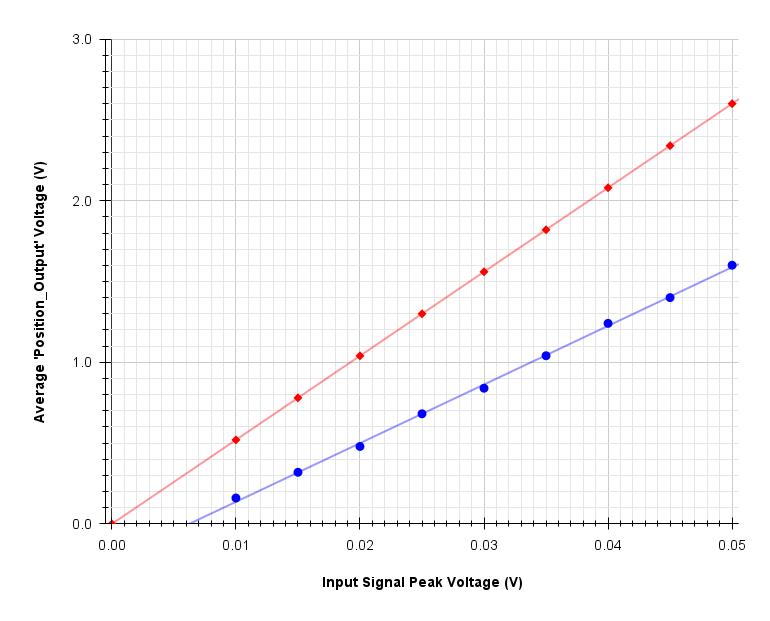
\includegraphics[width=1\linewidth]{graphs/555_fullrange.png}
    \caption[Design B: Input Range Response]{Graph of Design B Input Signal Peak Voltage (V) against observed `Position\_Output' (V). Average observed output voltage is represented in Blue, and predicted output voltage is represented in Red.}
    \label{fig:555_fullrange}
\end{figure}

Fig.\ref{fig:555_fullrange} demonstrates the relationship between the input peak voltage and the observed output voltage within Design B. As shown in Fig.\ref{fig:555_fullrange}, the output voltage increases proportionally with the input peak voltage, following a near-linear trend as expected for a fixed-gain non-inverting amplifier circuit. However, observed output values were consistently lower than the theoretical values predicted by the amplifier’s nominal gain setting of 52, indicating a reduction in observed gain within the circuit.

The maximum observed voltage was \(1.601\) V and a minimum observed voltage of \(0.160\) V. It should be noted that the linear trend does not cross through the origin but crosses the x-axis at \(\approx0.006\) V.

These observations confirm the amplifier's overall linear behaviour, highlighting the practical limitations demonstrated by the difference between the theoretical gain and observed gain.

\subsubsection{Cost of Implementation}

\begin{table}[H]
\centering
\caption{Alphabetically Ordered Estimated Component Costs for Design B}
\begin{tabular}{|l|c|c|c|}
\hline
\textbf{Component}                & \textbf{Quantity} & \textbf{Unit Price (£)} & \textbf{Total Price (£)}\\ \hline
100nF Ceramic Disc Capacitor\cite{rs_100nfcap} & 3 & 0.17 & 0.51\\ \hline
1kΩ Resistor \cite{rs_1kresistor} & 1 & 0.162 & 0.162\\ \hline
1μF Electrolytic Capacitor \cite{rs_1ufcap} & 1 & 0.218 & 0.218\\ \hline
1N4148 Diode \cite{rs_1n4148} & 1 & 0.01 & 0.01\\ \hline
2.2nF Ceramic Capacitor \cite{rs_2nfcap}& 1 & 0.068 & 0.068\\ \hline
33nF Polyester Capacitor  \cite{rs_33nfcap} & 1 & 0.12 & 0.12\\ \hline
4.7μF Electrolytic Capacitor \cite{rs_5ufcap}& 1 & 0.206 & 0.206\\ \hline
47kΩ Resistor \cite{rs_47kresistor}& 1 & 0.167 & 0.167\\ \hline
51kΩ Resistor \cite{rs_51kresistor} & 1 & £0.054 & £0.054\\ \hline
5.6kΩ Resistor \cite{rs_6kresistor}& 1 & 0.106 & 0.106\\ \hline
9V Battery (RS PRO Alkaline) \cite{rs_9vbattery} & 1 & 2.08 & 2.08 \\ \hline
10nF Polyester Capacitor \cite{rs_10nfcap} & 1 & 0.112 & 0.112\\ \hline
NE555P Timer IC \cite{rs_ne555p} & 1 & 0.152 & 0.152\\ \hline
TL071 Operational Amplifier \cite{rs_tl071} & 1 & 0.45 & 0.45\\ \hline\hline
\textbf{Total Estimated Cost} &&&\textbf{£4.41}\\ \hline
\end{tabular}
\label{tab:component_info_db}
\end{table}

Table \ref{tab:component_info_db} details the individual components required for the implementation of Design B, alongside their quantities, specifications, suppliers, and unit costs based on UK-sourced pricing at the time of writing. The cost of implementation within the `mouse' would be £5.54, adding an additional non-inverting amplifier and peak detector. The cost difference between the original sub-system (Appendix \ref{app:mouseecost_og}) is -£1.84 a reduction of \(25\%\). 

\section{Discussion}
This section covered the evaluation of three design solutions proposed to facilitate the operation of the position feedback system from a single DC supply of \(9\) V. Firstly, of the three designs assessed, two designs produced stable outputs when assembled, suggesting these are possible solutions to the dual power supply issue. Secondly, the output signals produced by the physical designs were of an observable voltage level that a microcontroller could utilise for position feedback. Thirdly, the cost of implementation is less than that of the current dual power supply operational amplifier circuit.

Before further interpreting the findings, we must note several important limitations. Firstly, the current methods do not account for varying temperatures. All tests were carried out at room temperature \(22\) \(\degree\)C. Changes in electrical characteristics could cause incorrect design behaviour due to an increase or decrease in device temperatures. This limitation should be considered when shrinking the circuit size down and concentrating components together, increasing potential heat interference from hot components, especially the MOSFETs (IRLZ44N). Secondly, no accommodation is made regarding the observed input signal amplitude and signal generator amplitude discrepancy. This could introduce uncertainty into the observed output DC voltages and the corresponding gain achieved. The primary project aim was to evaluate the linearity and efficacy between designs, rather than obtain absolute voltage values with high precision.  Thirdly, for consistency of results the \(9\) V power rail in Design A and B was provided with a laboratory power supply and not batteries, which will have a higher impedance especially as they discharge with use potentially impacting performance.

\subsubsection{Design Performance}
Design A and B provided consistent and reliable output voltages that linearly followed the input signal voltage. However, the observed `Position\_Output' voltage was lower than the amplifier output due to the voltage drop across the diode; this could be corrected by placing the diode inside the feedback loop. In addition, this would also remove any diode drop with temperature. Furthermore, the observed gain in both designs was lower than expected; however, this shouldn't be an issue in actual application, as variable resistors are used to match the signals, and additional Arduino scaling can be done to balance the left and right sensor signals.

\subsubsection{Complexity}
Design A is simple in background knowledge and requires only basic electrical engineering principles to integrate. In contrast, Design B has more complexity due to introducing difficult principles and complicated circuitry; however, documentation is available to guide the creation of Design B.

\subsubsection{Cost}
Both Design A and B provide a cost reduction from the original sub-system due to the expensive nature of batteries and the removal of one. Comparing the two designs to one another, Design B is slightly more cost-effective with a larger total cost reduction.

\subsubsection{Further Investigations}
Further evaluation should be conducted on Design A and B once integrated into a working `mouse', validating circuit performance with battery supplies and interaction with LC filter circuit. In addition, a set of secondary sensors on the rear of the `mouse' should be investigated, with the intention of using them to help identify straights and corners more effectively.

\subsubsection{Recommendations}
On the whole, both Design A and B are recommended as potential solutions to solve the dual power supply operational amplifier issue. Both designs have valid use cases and should be considered, however in the current state of the `mouse' project Design B is the final recommendation, costing less and having a greater operational range than Design A.




